\section{Results}\label{sec:results}

\subsection{The pool-injection contrast across libraries}

Table~\ref{tab:main} reports the pool-injection contrast, A1$-$A0, on the sealed panel of each library.
In the primary library the point estimates are $+2.02$ points under
AlexNet with a 95\% CI of $+0.83$ to $+3.35$, and $+1.70$ under Swin-T with CI $+1.28$ to
$+2.84$. Both intervals
exclude zero. Under the add-one convention, both smaller tails have zero hits in 2{,}000
resamples: raw $p=2/2{,}001$ and Holm-adjusted $p\approx0.0020$ for both, so the interval excludes zero in the primary
family at the finest resolution 2{,}000 resamples can express, the smallest attainable two-sided
tail being $2/2{,}001$, conditional on the fixed split and the trained seeds.
Both point estimates are, however, below the three-point SESOI recorded in the internal written
protocol, which the local record describes as set before training. The Swin-T interval is wholly below three points, whereas the AlexNet interval includes
that magnitude. These are conditional intervals for our fixed split and trained seeds, not
uncertainty bounds across new training runs or split realisations. A null-compatible interval is
not evidence of no effect, and we make no equivalence claim at any margin.

\begin{table}[t]
\centering
\caption{Main effect, A1$-$A0, on the sealed panel. A0 and A1 are macro-F1 on a 0--1 scale, the
latter with probability averaging followed by one vote per recording; the $\Delta$ columns and the
seed range are in percentage points. Recording-level points were corrected after the main runs;
their original unweighted cluster intervals are retained. Intervals are 95\% recording-cluster
bootstrap intervals over 2{,}000 resamples on the primary replicate stream; the class-set
comparison in Supplementary Material S1 re-draws them on a second stream, so its bounds differ in
the second decimal. Seed range is the spread of per-seed differences. The two primary rows, CTIS under both backbones, are marked with a dagger:
neither reaches the three-point threshold of the internal plan, whereas every additional-library
point estimate does; a point estimate falling short does not by itself mean its interval
excludes that magnitude. Differences
are computed on unrounded per-seed scores, so subtracting the four-decimal arm columns can differ
from the reported $\Delta$ by 0.01.}
\label{tab:main}
\scriptsize
\setlength{\tabcolsep}{1.5pt}
\begin{tabular}{l@{\hspace{3pt}}lrrrrr}
\toprule
Library & Backbone & A0 & A1 & $\Delta$ slice [95\% CI] & $\Delta$ rec. [95\% CI] & Seed \\
\midrule
CTIS        & AlexNet$^{\dagger}$ & 0.9078 & 0.9279 & $+2.02\;[+0.83,+3.35]$ & $+1.37\;[+0.26,+2.83]$ & 1.86 \\
CTIS        & Swin-T$^{\dagger}$  & 0.9536 & 0.9706 & $+1.70\;[+1.28,+2.84]$ & $+1.61\;[+0.87,+2.60]$ & 1.36 \\
music genre& AlexNet & 0.6889 & 0.8411 & $+15.22\;[+13.07,+17.53]$ & $+15.13\;[+11.97,+18.91]$ & 0.97 \\
music genre& Swin-T  & 0.7346 & 0.9145 & $+17.99\;[+15.29,+21.20]$ & $+15.98\;[+12.88,+19.78]$ & 0.89 \\
pianos      & AlexNet & 0.8237 & 0.9699 & $+14.62\;[+11.89,+18.28]$ & $+7.53\;[+3.90,+12.26]$ & 2.07 \\
pianos      & Swin-T  & 0.8699 & 0.9835 & $+11.36\;[+8.15,+15.26]$ & $+4.86\;[+2.07,+8.43]$ & 3.21 \\
CNPM        & AlexNet & 0.4066 & 0.6304 & $+22.39\;[+14.60,+29.99]$ & $+28.44\;[+17.82,+38.70]$ & 7.13 \\
CNPM        & Swin-T  & 0.4002 & 0.6873 & $+28.71\;[+19.75,+37.52]$ & $+30.75\;[+21.66,+39.57]$ & 2.71 \\
bel canto & AlexNet & 0.8200 & 0.9043 & $+8.42\;[+5.18,+13.80]$ & $+14.61\;[+5.71,+26.23]$ & 2.46 \\
bel canto & Swin-T  & 0.8091 & 0.9397 & $+13.06\;[+7.50,+24.75]$ & $+22.74\;[+9.28,+41.28]$ & 2.96 \\
\bottomrule
\end{tabular}
\end{table}

In the four additional libraries the same manipulation moves macro-F1 by $+8.4$ to $+28.7$
points, compared with $+2.02$ (AlexNet) and $+1.70$ (Swin-T) in CTIS. Baseline headroom differs
substantially; the similar library medians of exposure alone do not establish its role in the
between-library spread. CTIS starts
from 0.908 under AlexNet and 0.954 under Swin-T, so at most 9.2 and 4.6 points were available to
be won, and the observed gains consume 22\% and 37\% of that headroom. Expressed as a share of
the remaining score headroom, the effects span 22--87\%, as Table~\ref{tab:headroom} shows.
This normalisation is descriptive, not a decomposition of mechanisms.

The CTIS-only C1 control, defined in Section~\ref{sec:protocol}, checks equal-volume
replacement with non-test content. C1 and A1 differ primarily in the origin of injected content,
but also in recording diversity and the use of validation recordings. Because C1 consumes R content, its validation scores cannot be interpreted, and every C1 number below is a sealed-panel score. C1
trains on 25{,}502 slices against 25{,}498 for A1 and 25{,}502 for A0, and the per-class counts are
unchanged. On the sealed panel C1$-$A0 is $+0.05$ $[-0.94,+1.35]$ under AlexNet and $+0.62$
$[+0.14,+1.81]$ under Swin-T, against $+2.02$ and $+1.70$ for A1$-$A0. Under Swin-T the C1$-$A0
interval excludes zero as well, so equal-volume non-test injection is not by itself equivalent to
the control, while the point estimate also falls below the three-point SESOI. Equal-volume non-homologous
content changes the slice-level point estimates by about 0.6 points or less, 3\% and 36\% of the respective
A1 point estimates. Comparing the two arms directly, as a paired contrast on the same sealed panel
and the same three seeds, the exposure arm still leads: A1$-$C1 is $+1.96$ points, 95\% CI $+0.74$
to $+2.99$, under AlexNet and $+1.07$, $+0.23$ to $+1.96$, under Swin-T at slice level, and
$+1.23$ $[+0.04,+2.13]$ and $+1.17$ $[+0.13,+2.09]$ at recording level. All four intervals exclude
zero and none reaches three points, so the difference between the two arms is smaller than the
A0 contrast but is not explained by resampling noise alone. The C1--A1 comparison remains
descriptive, not an additive decomposition of the A1 effect into exposure and diversity, and it
does not separate within-recording exposure from the additional pool recordings that A1 also
contains. C1 was added after the main design and is exploratory.

A second exploratory split goes at the same question from the recording side. The frozen split
files identify 578 of the 963 CTIS test recordings that contribute at least one slice to the
injected pool; the other 385 contribute none, so for them A1 differs from A0 only through the
additional pool recordings and the content that arrives with them. Grouping the sealed panel this
way, the A1$-$A0 contrast is larger where the test recording itself reached training: at slice
level $+4.03$ $[+2.69,+6.14]$ for the 578 exposed recordings under AlexNet against $-0.19$
$[-1.81,+1.83]$ for the remaining 385, and at recording level $+3.81$ $[+1.76,+5.36]$ against
$+0.27$ $[-1.67,+1.99]$; under Swin-T the same split gives $+2.67$ $[+1.71,+3.64]$ against
$+1.10$ $[+0.27,+3.04]$ at slice level and $+1.73$ $[+0.71,+2.58]$ against $+0.70$
$[-0.16,+2.28]$ at recording level. The pattern is therefore suggestive, not clean. The subgroup without any exposed
recording is small---710 slices and 385 recordings---and its Swin-T slice-level interval
excludes zero; the two subgroups are also re-clustered and resampled
separately, so their class universes differ and their absolute values are not comparable to each
other or to the pooled estimate. This split was computed after the main runs and is not part of the
internal plan.

\begin{table}[t]
\centering
\caption{The effect rescaled by the headroom available. Headroom is $100 - \mathrm{A0}$ in
points; the last column is the point estimate of $\Delta$ divided by headroom, i.e.\ the share of
the baseline's remaining score headroom. This is not a fraction of misclassified examples. Libraries with a high baseline cannot
express a large absolute gain, so the absolute column of Table~\ref{tab:main} and this column
must be read together.}
\label{tab:headroom}
\small
\begin{tabular}{llrrr}
\toprule
Library & Backbone & Headroom, pts & $\Delta$, pts & $\Delta/$headroom \\
\midrule
CTIS        & AlexNet &  9.22 &  2.02 & 0.219 \\
CTIS        & Swin-T  &  4.64 &  1.70 & 0.366 \\
music genre & AlexNet & 31.11 & 15.22 & 0.489 \\
music genre & Swin-T  & 26.54 & 17.99 & 0.678 \\
pianos      & AlexNet & 17.63 & 14.62 & 0.829 \\
pianos      & Swin-T  & 13.01 & 11.36 & 0.873 \\
CNPM        & AlexNet & 59.34 & 22.39 & 0.377 \\
CNPM        & Swin-T  & 59.98 & 28.71 & 0.479 \\
bel canto  & AlexNet & 18.00 &  8.42 & 0.468 \\
bel canto  & Swin-T  & 19.09 & 13.06 & 0.684 \\
\bottomrule
\end{tabular}
\end{table}

The CTIS sensitivity analyses in Supplementary Material S1 retain positive slice-level
intervals when recording clusters and trained seeds are jointly resampled. Some upper bounds
exceed three points: +3.74 under AlexNet and +3.14 under Swin-T on unstratified joint
seed--recording resampling. For the corrected
recording metric, AlexNet's unstratified joint interval includes zero, at approximately
$-0.03$ to $+2.99$. These exploratory analyses do not include split-realisation variance.

The two metric levels need not agree. In pianos the recording-level A1 contrasts are
$+7.53$ and $+4.86$ points, substantially smaller than the slice-level $+14.62$ and $+11.36$.
Probability averaging and equal recording weights alter the metric, so this is not proof of a
particular leakage mechanism. In bel canto the corrected recording-level contrasts are
$+14.61$ and $+22.74$, with broad intervals; only 40 test recordings are available, compared
with 54 in CNPM. Those small panels limit precision. For CTIS A2 under AlexNet the corrected
recording-level contrast is $+0.23$ with interval $[-0.95,+1.69]$, so it does not exclude zero.
Supplementary Material S1 reports the correction and training-seed sensitivity explicitly.

\subsection{Reconstructing a slice-level split usually yields a smaller sealed-panel contrast}

A2 varies two things at once --- it moves slices of pooled recordings into training, and it does so
through a random 80/10/10 partition of the pooled corpus. Its difference from A0 is therefore
usually smaller than A1's, because the random partition places only a fraction of the pool in
training, and its self-test score, not its sealed-panel score, is the one a user of the stated ratio would
print under a slice-level reading. As a
share of the pool-injection contrast, the
answer, in Table~\ref{tab:a2}, is $100\times\hat\Delta_{A2}/\hat\Delta_{A1} = 60$--103\%: in the
four additional libraries this reconstruction recovers between 81\% and 99\% of the A1 effect,
whereas in the primary library the recovered share spans the two extremes of the ten: 60\%
under AlexNet and 103\% under Swin-T. In CTIS under AlexNet the interval touches zero, at $+1.21$
with CI $-0.02$ to $+2.44$ and $p = 0.056$, so the reconstruction is not reliably better than the
control arm there; under Swin-T it is, at $+1.75$ with CI $+1.18$ to $+2.70$. The A2 self-test scores --- an illustrative stand-in for the score this reconstruction
would print under a slice-level reading --- are shown as open squares in Figure~\ref{fig:arms} and sit above every other
point in every library. Self-test slices are disjoint from training slices, but may come from
the same recordings; the panels and their supports differ, and in one library a small number of
self-test images repeat content that also appears in A2 training (Supplementary Material S1). A self-test-minus-A0 difference is
therefore descriptive, not a paired estimate of leakage. Supplementary Material S1 reports the
self-test scores and seed dispersion explicitly.

\begin{table}[t]
\centering
\caption{Our reconstruction of a slice-level split, A2$-$A0; the slice-level and recording-level
columns report the two levels. A2 trains on a random 80/10/10 split of C $\cup$ $Q^{\text{pool}}$, i.e.\ with
same-recording mixing; its realised training count is 0.991--1.001 of A0's in every library.
Intervals are conditional 95\% recording-cluster bootstrap intervals (2{,}000 resamples).
The self-test scores are tabulated separately in Supplementary Material S1. In bel canto under
Swin-T, A1 and A2 both reach 1.00 at the recording level in every seed while A0 averages 0.77, so
their contrast and interval coincide by construction.}
\label{tab:a2}
\small
\begin{tabular}{llrr}
\toprule
Library & Backbone & $\Delta$ slice [95\% CI] & $\Delta$ recording [95\% CI] \\
\midrule
CTIS        & AlexNet & $+1.21\;[-0.02,+2.44]$ & $+0.23\;[-0.95,+1.69]$ \\
CTIS        & Swin-T  & $+1.75\;[+1.18,+2.70]$ & $+1.77\;[+0.89,+2.65]$ \\
music genre & AlexNet & $+14.06\;[+12.19,+16.14]$ & $+13.93\;[+10.96,+17.55]$ \\
music genre & Swin-T  & $+16.52\;[+14.16,+19.39]$ & $+15.40\;[+12.31,+19.19]$ \\
pianos      & AlexNet & $+14.07\;[+11.48,+17.65]$ & $+7.77\;[+4.23,+12.50]$ \\
pianos      & Swin-T  & $+11.23\;[+8.09,+15.13]$ & $+5.10\;[+2.18,+8.91]$ \\
CNPM        & AlexNet & $+18.07\;[+10.48,+26.13]$ & $+24.94\;[+15.35,+34.28]$ \\
CNPM        & Swin-T  & $+26.76\;[+17.01,+35.66]$ & $+34.04\;[+24.52,+43.62]$ \\
bel canto  & AlexNet & $+7.30\;[+4.46,+11.98]$ & $+17.05\;[+6.47,+31.17]$ \\
bel canto  & Swin-T  & $+12.51\;[+7.00,+24.54]$ & $+22.74\;[+9.28,+41.28]$ \\
\bottomrule
\end{tabular}
\end{table}

\begin{figure}[!tb]
\centering
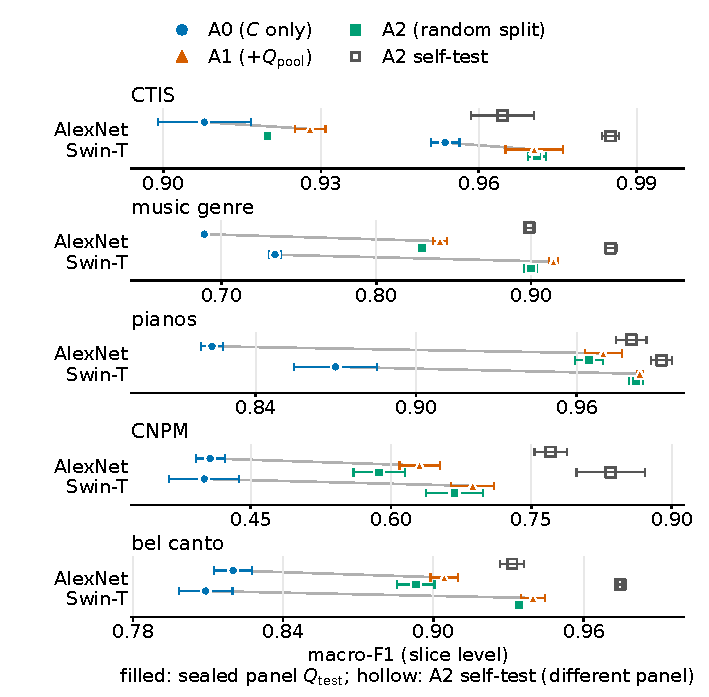
\includegraphics[width=\linewidth]{../figures/fig4_three_arms.pdf}
\caption{Sealed-panel macro-F1 at slice level for the three main arms; the five libraries form the
panels and the two backbones the rows. Circles: A0, which sees no test-adjacent content. Triangles: A1, into which the
held-out pool is injected by equal replacement. Filled squares: A2, our reconstruction of a
slice-level split.
Open squares: A2's own self-test score, drawn slightly above the row for legibility without
changing its horizontal value. It uses a different panel, not the sealed test panel.
Within each row the three arms are dodged vertically (A0 highest, A2 lowest) so that arms
whose scores coincide stay distinguishable; vertical position carries no quantitative meaning.
Horizontal whiskers are $\pm1$ sample standard deviation over three training seeds, not a
confidence interval and not the paired interval in Table~\ref{tab:main}. Horizontal segments span A0 to A1. Note that the horizontal axis is scaled per
library: the five baselines span 0.40 to 0.95, and a shared axis would compress the primary
library's two-point difference to invisibility.}
\label{fig:arms}
\end{figure}

\subsection{Near-single-slice controls as pipeline sanity checks}

Six A0 versus A2 contrasts on the three usable K$\approx$1 libraries, each with three seeds, give
five intervals that include zero, as Table~\ref{tab:neg} lists, and the intervals are narrow: apart from
one cell their outer bounds lie within about four points of zero. The remaining cell, chest\_falsetto
under Swin-T, is the only negative departure and the only interval that excludes zero
at $-2.53$ with CI $-5.00$ to $-0.21$; its per-seed deltas are $+5.57$, $-2.62$ and $-10.54$, so its 16.1-point
seed range is larger than the effect itself. The signs differ across the three trained seeds,
so this conditional interval does not establish a stable direction across training runs. The expansion from one
to three seeds was exploratory, not publicly preregistered. GZ\_IsoTech, the only control with multi-segment recordings, sits at $+0.26$ and $-0.22$,
consistent with its sub-one-percent exposure. Because A2 is not the main intervention, these cells
do not test A1$-$A0 directly and cannot bound uncertainty in the main experiment.
With six contrasts and no correction for multiplicity, the single nominal exclusion is itself weak
evidence, and five intervals that include zero do not show that the contrast is zero.
Recording- and slice-level partitions coincide only in the exactly single-slice collections,
so these are pipeline checks rather than evidence isolating a universal leakage mechanism.

\begin{table}[t]
\centering
\caption{Negative controls: A0 versus A2 on libraries with roughly one slice per recording, three
seeds. With one slice per recording there is no homologous content, so the exposure arm is not
identifiable and A2 is the only arm that can differ; the contrast column therefore measures protocol
noise rather than leakage. Five of the six intervals include zero. The remaining one is the only
negative departure, chest\_falsetto under Swin-T at $-2.53$, and its seed range of 16.1 points shows
substantial sensitivity to the three trained seeds. The six contrasts are reported without a
correction for multiplicity, and five intervals that include zero are not an equivalence test:
they do not establish that the protocol contrast is zero. This does not establish the cause of the
non-zero conditional interval. Intervals are 95\% recording-cluster bootstrap intervals
(2{,}000 resamples) conditional on the fixed seeds and split.}
\label{tab:neg}
\footnotesize
\setlength{\tabcolsep}{3.6pt}
\begin{tabular}{llrrrr}
\toprule
Library & Backbone & Rec.\, /\, slices & $\Delta$ [95\% CI] (pts) & Seed range (pts) & Tail prop. \\
\midrule
chest\_falsetto     & AlexNet & 1{,}280 / 1{,}280 & $-1.37\;[-3.31,+0.56]$ & 4.29  & 0.167 \\
chest\_falsetto     & Swin-T  & 1{,}280 / 1{,}280 & $-2.53\;[-5.00,-0.21]$ & 16.12 & 0.036 \\
erhu\_playing\_tech & AlexNet & 1{,}253 / 1{,}253 & $+0.03\;[-1.14,+1.24]$ & 2.54  & 0.928 \\
erhu\_playing\_tech & Swin-T  & 1{,}253 / 1{,}253 & $-0.49\;[-1.93,+0.40]$ & 1.93  & 0.382 \\
GZ\_IsoTech         & AlexNet & 2{,}824 / 2{,}899 & $+0.26\;[-0.23,+0.87]$ & 0.26  & 0.381 \\
GZ\_IsoTech         & Swin-T  & 2{,}824 / 2{,}899 & $-0.22\;[-0.56,+0.05]$ & 0.74  & 0.163 \\
\bottomrule
\end{tabular}
\end{table}

\subsection{Technique classification performance decreases on held-out instruments}

The cross-instrument experiment gives the largest contrast in the study and the one most
useful for interpreting published technique-classification numbers. With random slice-level
folds, pooled macro-F1 on CTIS techniques reaches 0.845 under AlexNet and 0.877 under Swin-T.
Grouping the folds by instrument --- same data, same budget, but every test recording's
instrument withheld from training --- brings the same pipeline to 0.448 and 0.530. The difference is $+39.6$ points
$[+36.8,+42.4]$ under AlexNet and $+34.8$ points $[+32.0,+38.1]$ under Swin-T, as
Table~\ref{tab:p3} reports.

Two things change between those two arms, so we added a third partition, R-rec, that
provides an operational intermediate comparison: folds are grouped by recording, with 110
instruments appearing on at least two folds. Thus most instrument overlap is retained while
recording overlap is removed, but not every instrument is present in every training/test pair.
Recording-grouped partitions are feasible on this corpus: no recording and no duplicate-audio group
crosses a fold, all 43 classes keep at least one test recording in the recording-grouped partition,
and fold sizes differ by less than 0.1\%. The instrument-withheld partition is tighter: its first
fold covers 42 of the 43 classes, because one technique class has no test recording there, and the
pooled metric averages only over classes present. The class universe itself comes from a
study-specific rule stated in Section~\ref{sec:protocol}: technique--instrument cells with at least
two recordings and instruments contributing at least three recordings, after excluding six
content-type labels. The R-rec partition reaches 0.816
and 0.843, so removing the recording-level leak lowers macro-F1 by $2.90$ points
(CI $0.32$ to $5.66$) under AlexNet and $3.41$ points (CI $0.68$ to $6.36$) under Swin-T.
Withholding the instruments then lowers it by a further $36.7$ points ($33.3$ to $39.9$) and
$31.4$ points ($28.3$ to $35.0$). The large number in
Table~\ref{tab:p3} is therefore two effects of very different size: within-instrument
the R-slice--R-rec contrast is 7--10\% of the total, with the larger remainder in the
R-rec--L-inst contrast. This separates protocol contrasts rather than decomposing
all sources of performance loss: neither the 36.7-point (AlexNet) or 31.4-point (Swin-T)
R-rec--L-inst gap nor the 39.6-point or 34.8-point R-slice--L-inst gap is a leakage estimate.
Figure~\ref{fig:p3} shows the
four partitions side by side with their intervals.

\begin{figure}[!tb]
\centering
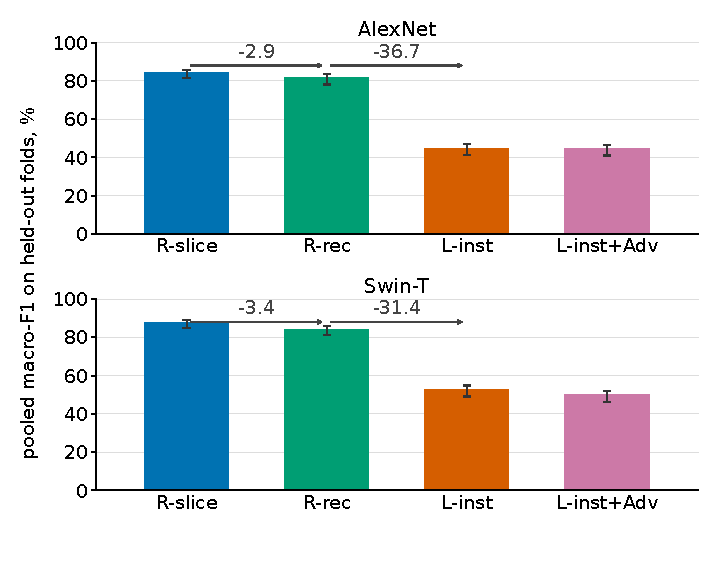
\includegraphics[width=\linewidth]{../figures/fig2_p3_decomposition.pdf}
\caption{Separating recording-disjoint and instrument-withheld protocol contrasts. Pooled macro-F1 on
held-out folds of the CTIS technique task for four partitions: random slice-level folds (R-slice),
recording-grouped folds with 110 instruments on at least two folds (R-rec),
instrument-withheld folds (L-inst), and the adversarial arm on the same folds (L-inst+Adv). Bars are means over
two seeds and the whiskers are 95\,\% recording-cluster bootstrap intervals. The two arrows
give the R-rec$--slice contrasts of $-2.9$ and $-3.4$ points and the
L-inst$--rec contrasts of $-36.7$ and $-31.4$ points, for AlexNet and Swin-T in that
order. They are differences between
protocols, not causal components of a single mechanism.}
\label{fig:p3}
\end{figure}

The adversarial instrument head does not recover the loss relative to L-inst. Under AlexNet it changes pooled
macro-F1 by $-0.36$ $[-1.75,+0.91]$; under Swin-T it changes it by $-2.83$ $[-4.81,-0.89]$.
The instrument-identity probe, fitted on a closed set of the instrument classes present in the
training recordings, shows that this information remains decodable: on frozen features
it reaches AUC 0.94 for R-slice and 0.96 for L-inst, and the adversarial head lowers it only
to 0.93 for L-inst+Adv while technique macro-F1 falls. Because the probe is fitted on an 80/20
split of the training recordings and its class set is closed, it measures how much instrument
identity remains recoverable for instruments the model has seen; it does not establish that an
unseen test instrument is identifiable from the representation. These rounded summaries are pooled across
folds, seeds and both backbones; Supplementary Material S1 gives the backbone-specific probe values.
The gradient-reversal weight was at most 0.02. The adversarial and L-inst arms use the same
instrument-grouped folds; they
differ in the objective, not the recordings seen.
This is a negative result for this intervention and weight schedule, not evidence that
instrument invariance is unattainable.

\begin{table}[t]
\centering
\caption{Cross-instrument transfer on CTIS techniques, over 43 classes, 1{,}388 recordings and
7{,}528 slices in three folds with two seeds, pooled over the held-out folds. R-slice uses random slice-level folds and
is the optimistic within-recording reference; R-rec groups folds by recording while retaining overlap for 110 instruments on at least two folds; L-inst withholds whole instruments; L-inst+Adv adds an adversarial instrument head on top of
L-inst. The recording-level column for R-slice aggregates slice predictions from more than one
fold model, so it is not directly comparable with the single-model recording-level column of the
other partitions. Intervals are 95\% recording-cluster bootstrap intervals. Contrasts on the pooled slice metric: R-slice$-$L-inst
$+39.63\,[+36.84,+42.39]$ for AlexNet and $+34.77\,[+32.00,+38.08]$ for Swin-T; R-slice$-$R-rec
$+2.90\,[+0.32,+5.66]$ and $+3.41\,[+0.68,+6.36]$; R-rec$-$L-inst
$+36.73\,[+33.31,+39.89]$ and $+31.37\,[+28.32,+34.97]$; L-inst+Adv$-$L-inst $-0.36\,[-1.75,+0.91]$ for AlexNet
and $-2.83\,[-4.81,-0.89]$ for Swin-T. Contrasts use unrounded scores and can
differ from the difference of the four-decimal columns by 0.01.}
\label{tab:p3}
\footnotesize
\setlength{\tabcolsep}{3.6pt}
\begin{tabular}{llrr}
\toprule
Arm & Backbone & Pooled macro-F1, slice & Pooled macro-F1, rec. \\
\midrule
R-slice         & AlexNet & 0.8446 & 0.8797 \\
R-slice         & Swin-T  & 0.8772 & 0.9041 \\
R-rec & AlexNet & 0.8157 & 0.8640 \\
R-rec & Swin-T  & 0.8431 & 0.8799 \\
L-inst & AlexNet & 0.4483 & 0.4917 \\
L-inst & Swin-T  & 0.5295 & 0.5676 \\
L-inst+Adv      & AlexNet & 0.4447 & 0.4714 \\
L-inst+Adv      & Swin-T  & 0.5012 & 0.5467 \\
\bottomrule
\end{tabular}
\end{table}

\subsection{Compute}

The final main comparison contains 60 A0/A1 training runs and 30 A2 runs. The expanded
negative controls contain 36 runs, the CTIS-only C1 control six runs, and the cross-instrument
experiment 48 fold-models including the recording-grouped intermediate arm. Driver timings
are rounded wall-clock batch durations on one 16 GB GPU, not independently metered GPU-hours.
Available logs indicate about 6.25 h for A0/A1, 4.15 h for A2, 2.99 h for the cross-instrument
fold-models and 1.17 h for C1; an additional recording-grouped/probe driver records about
0.55 h. Negative-control timing and abandoned exploratory runs are incompletely recoverable.
We therefore report the partial ledger in Supplementary Material S1, not an exact full-study
cost. Rebuilding recording identifiers and splits itself does not require a GPU.
